% Opinion-Guided Valence-Arousal Prediction for Dimensional Aspect Sentiment Quad Prediction
% Target: ICONIP 2026 (Springer LNCS format, 10-12 pages)

\documentclass[runningheads]{llncs}

\usepackage[T1]{fontenc}
\usepackage{graphicx}
\usepackage{amsmath,amssymb}
\usepackage{booktabs}
\usepackage{multirow}
\usepackage{tikz}
\usetikzlibrary{positioning, arrows.meta, shapes.geometric, fit, calc, backgrounds, decorations.pathreplacing}
\usepackage{pgfplots}
\pgfplotsset{compat=1.18}
\usepackage{xcolor}
\usepackage{subcaption}
\usepackage{algorithm}
\usepackage{algpseudocode}
\usepackage{hyperref}

% Custom colors (pre-defined to avoid xcolor inline mixing issues with llncs)
\definecolor{encoderblue}{RGB}{66,133,244}
\definecolor{matrixgreen}{RGB}{52,168,83}
\definecolor{vahead}{RGB}{234,67,53}
\definecolor{priorpurple}{RGB}{142,68,173}
\definecolor{gateorange}{RGB}{243,156,18}
\definecolor{lightgray}{RGB}{245,245,245}
% Mixed colors for TikZ architecture diagram
\definecolor{darkgray}{RGB}{130,130,130}
\definecolor{medgray}{RGB}{160,160,160}
\definecolor{arrowgray}{RGB}{100,100,100}
\definecolor{dashgray}{RGB}{128,128,128}
\definecolor{inputborder}{RGB}{170,170,170}
\definecolor{inputfill}{RGB}{242,242,242}
\definecolor{encoderbluefill}{RGB}{210,228,252}
\definecolor{vaheadfill}{RGB}{253,224,221}
\definecolor{vaheadborder}{RGB}{244,161,149}
\definecolor{vaheadlightfill}{RGB}{254,245,244}
\definecolor{matrixgreenfill}{RGB}{218,241,221}
\definecolor{priorpurplefill}{RGB}{235,220,243}
\definecolor{gateofill}{RGB}{253,239,213}
\definecolor{ebluefill}{RGB}{222,236,254}
\definecolor{ppfill}{RGB}{238,226,245}
\definecolor{concatfill}{RGB}{240,240,240}
\definecolor{resborder}{RGB}{110,110,110}
\definecolor{resfill}{RGB}{235,235,235}

\begin{document}

\title{Opinion-Guided Valence-Arousal Prediction\\for Dimensional Aspect Sentiment Quad Extraction}

% Authors anonymized for review
\author{Anonymous Authors}
\institute{Anonymous Institution}

\maketitle

%==============================================================================
\begin{abstract}
% SCQA: Situation → Conflict → Question → Answer
%
% S: Dimensional Aspect-Based Sentiment Analysis (DimABSA) extends traditional
%    ABSA by replacing discrete polarity labels with continuous
%    Valence-Arousal (VA) scores, enabling finer-grained sentiment modeling.
% C: Existing token-pair matrix methods for aspect sentiment quad prediction
%    predict VA values at the token level, ignoring the dependency of VA on
%    specific aspect-opinion interactions and the inherent sentiment prior
%    carried by opinion expressions.
% Q: How can we effectively leverage opinion-level sentiment priors while
%    conditioning VA prediction on aspect-opinion pair context?
% A: We propose Opinion-Guided VA, a gated residual mechanism that decomposes
%    VA prediction into an opinion-derived prior and a context-dependent
%    residual, achieving significant VA quality improvements.

Dimensional Aspect-Based Sentiment Analysis (DimABSA) advances traditional ABSA by replacing discrete polarity labels with continuous Valence-Arousal (VA) scores, enabling fine-grained sentiment quantification. The Dimensional Aspect Sentiment Quad Prediction (DimASQP) task further requires jointly extracting aspect terms, opinion expressions, aspect categories, and their associated VA values from review texts. While token-pair matrix methods achieve competitive extraction performance, their token-level VA prediction ignores two critical factors: the dependency of sentiment intensity on specific aspect-opinion interactions, and the inherent VA prior carried by opinion expressions (e.g., ``\emph{delicious}'' inherently conveys high valence regardless of the aspect it modifies). We propose \textbf{Opinion-Guided VA prediction}, a gated residual mechanism that decomposes VA estimation into an opinion-derived prior and a context-dependent residual, integrated within a one-stage quad extraction framework. Experiments on two English benchmark domains show that our method significantly reduces VA prediction error (MAE\textsubscript{V} by 13.2\%, Euclidean distance by 9.6\% on restaurant data; $p<0.001$) while maintaining extraction performance, demonstrating that explicit modeling of opinion sentiment priors is an effective inductive bias for dimensional sentiment prediction.

\keywords{Dimensional Aspect-Based Sentiment Analysis \and Valence-Arousal Prediction \and Aspect Sentiment Quad Prediction \and Opinion-Guided Learning}
\end{abstract}

%==============================================================================
\section{Introduction}
\label{sec:intro}

Aspect-Based Sentiment Analysis (ABSA) aims to identify fine-grained sentiment expressed toward specific aspects in text~\cite{pontiki2016semeval}. While conventional ABSA tasks model sentiment as discrete polarities (positive, negative, neutral), this categorical representation fails to capture nuanced differences in sentiment intensity---for instance, ``\emph{amazing}'' and ``\emph{acceptable}'' both convey positive sentiment, yet differ substantially in emotional intensity.

Dimensional Aspect-Based Sentiment Analysis (DimABSA)~\cite{dimabsa2026} addresses this limitation by adopting the psychological Valence-Arousal (VA) model~\cite{russell1980circumplex}, where sentiment is represented as two continuous values: \emph{valence} (pleasantness, $V \in [1,9]$) and \emph{arousal} (activation, $A \in [1,9]$). This enables quantitative comparison of sentiment intensities and captures emotions that discrete labels cannot distinguish.

The most comprehensive formulation in this direction is \textbf{Dimensional Aspect Sentiment Quad Prediction (DimASQP)}, which requires extracting quadruplets $(a, c, o, \langle v, a \rangle)$ where $a$ is an aspect term, $c$ is an aspect category, $o$ is an opinion expression, and $\langle v, a \rangle$ are continuous VA values. The task is evaluated using Continuous F1 (cF1)~\cite{dimabsa2026}, which penalizes VA prediction errors through Euclidean distance weighting---even with perfect extraction, inaccurate VA predictions significantly degrade the final score.

Token-pair matrix methods~\cite{gao2023oneasqp} have proven effective for structured quad extraction by encoding span-pair relationships in a two-dimensional matrix. However, existing approaches predict VA values at the \emph{token level}, which introduces two fundamental limitations:
\begin{enumerate}
    \item \textbf{Quad ambiguity}: A single token may participate in multiple quadruplets with different VA values (e.g., ``\emph{food}'' in both a quality-related and a price-related quad), yet token-level prediction cannot disambiguate these cases.
    \item \textbf{Ignored opinion priors}: Opinion expressions carry inherent sentiment information---``\emph{terrible}'' strongly implies low valence regardless of what aspect it modifies---but token-level VA heads do not explicitly model this prior.
\end{enumerate}

We propose \textbf{Opinion-Guided VA prediction}, a simple yet effective mechanism that addresses both limitations. Our approach decomposes VA prediction into two components: (1)~an \emph{opinion prior} derived solely from the opinion span, capturing the base sentiment conveyed by the opinion expression; and (2)~a \emph{context-dependent residual} computed from the interaction between aspect and opinion representations, capturing how the aspect modulates the opinion's sentiment. A learnable gate balances these two components. This design provides an explicit inductive bias that opinion expressions are the primary carriers of VA information, while aspect context serves as a modulator.

Our contributions are as follows:
\begin{itemize}
    \item We propose Opinion-Guided VA prediction, a gated prior-residual mechanism for dimensional sentiment estimation within a one-stage quad extraction framework.
    \item We provide a thorough ablation study with three VA prediction architectures (token-level, span-pair conditioned, and opinion-guided), demonstrating that explicit opinion prior modeling is the key factor driving VA quality improvement.
    \item We present comprehensive analysis including learned gate behavior, statistical significance tests, and per-category VA error breakdowns, providing interpretable evidence for \emph{why} the method works.
\end{itemize}

%==============================================================================
\section{Related Work}
\label{sec:related}

\subsection{Aspect Sentiment Quad Prediction}

Aspect Sentiment Quad Prediction (ASQP) requires extracting all $(a, c, o, s)$ quadruplets from text, where $s$ denotes sentiment polarity. Approaches fall into two paradigms: \emph{generative methods} that formulate ASQP as sequence-to-sequence generation~\cite{zhang2021paraphrase,gou2023mvp}, and \emph{extractive methods} that use structured prediction over token pairs~\cite{gao2023oneasqp}. One-ASQP~\cite{gao2023oneasqp} introduced a token-pair matrix approach with EfficientGlobalPointer~\cite{su2022globalpointer}, decomposing quad extraction into parallel aspect-category detection and aspect-opinion-sentiment-category joint extraction. Our work extends this extractive framework to the dimensional setting.

\subsection{Dimensional Sentiment Analysis}

The shift from categorical to dimensional sentiment representations has gained momentum with shared tasks such as SIGHAN 2024 dimABSA and SemEval-2026 DimABSA~\cite{dimabsa2026}. HITSZ-HLT~\cite{hitszSighan2024} achieved top performance at SIGHAN 2024 with a hybrid BERT-LLM approach. CL-Span~\cite{clspanSighan2024} enhanced span representations with contrastive learning for VA prediction. Recent SemEval-2026 systems predominantly adopt LLM-based approaches, such as SCSG~\cite{scsg2026} using structured generation with self-consistency. Our work demonstrates that carefully designed VA prediction heads within lightweight encoder-based extractors remain competitive.

\subsection{Opinion-Sentiment Relationship}

The intuition that opinion expressions carry strong sentiment signals is well-established in ABSA. Opinion term extraction has been studied as an auxiliary task that benefits aspect-level sentiment classification~\cite{fan2019target,chen2020synchronous}. However, the explicit use of opinion representations as \emph{sentiment priors} for continuous VA prediction has not been explored. Our opinion-guided mechanism provides a principled way to leverage this intuition in the dimensional setting.

%==============================================================================
\section{Problem Definition}
\label{sec:problem}

Given an input text $\mathbf{x} = (x_1, x_2, \ldots, x_n)$, the DimASQP task requires extracting a set of quadruplets $\mathcal{Q} = \{(a_i, c_i, o_i, \langle v_i, a_i \rangle)\}_{i=1}^{|\mathcal{Q}|}$, where:
\begin{itemize}
    \item $a_i$ is an aspect term (a text span from $\mathbf{x}$, or \texttt{NULL} if implicit),
    \item $c_i \in \mathcal{C}$ is an aspect category from a predefined taxonomy,
    \item $o_i$ is an opinion expression (a text span, or \texttt{NULL} if implicit),
    \item $v_i \in [1, 9]$ and $a_i \in [1, 9]$ are valence and arousal scores.
\end{itemize}

\noindent\textbf{Evaluation.}\quad The official metric is Continuous F1 (cF1). Predicted and gold quadruplets are matched by exact string match on $(a, c, o)$. For each matched pair, a continuous true-positive score is computed as:
\begin{equation}
    \text{cTP} = \max\left(0,\; 1 - \frac{\sqrt{(v_p - v_g)^2 + (a_p - a_g)^2}}{\sqrt{128}}\right)
    \label{eq:ctp}
\end{equation}
where $\sqrt{128} \approx 11.31$ is the maximum possible Euclidean distance in the VA space. The cF1 is then computed as the harmonic mean of $\text{cPrecision} = \sum \text{cTP} / (|\text{TP}| + |\text{FP}|)$ and $\text{cRecall} = \sum \text{cTP} / (|\text{TP}| + |\text{FN}|)$.

%==============================================================================
\section{Method}
\label{sec:method}

\subsection{Overview}

Our framework builds upon the One-ASQP~\cite{gao2023oneasqp} architecture, extending it with a dedicated VA prediction head for dimensional sentiment estimation. As illustrated in Fig.~\ref{fig:architecture}, the system consists of three components: (1)~a pre-trained encoder that produces contextualized token representations; (2)~a token-pair matrix head that jointly extracts aspect terms, opinion expressions, and aspect categories; and (3)~an Opinion-Guided VA head that predicts continuous VA values conditioned on extracted span pairs.

\begin{figure}[t]
    \centering
    % Architecture diagram for Opinion-Guided VA Prediction
% Professional conference figure style: minimal colors, clean hierarchy
% Colors defined in main.tex

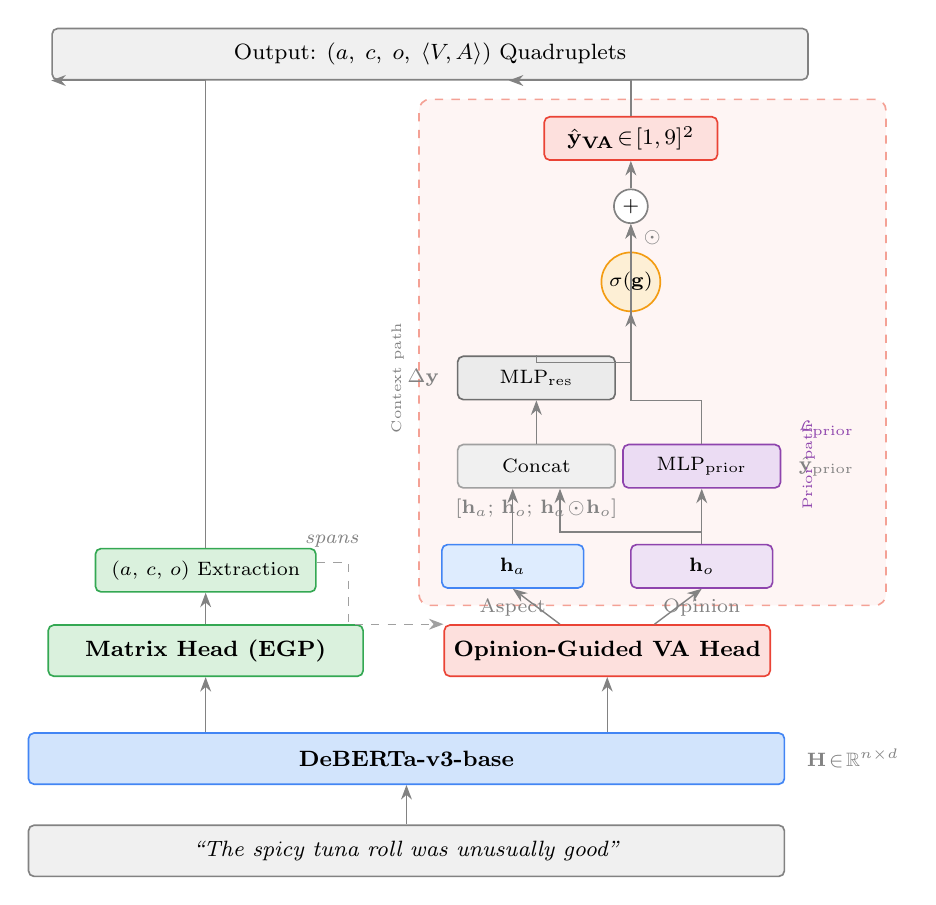
\begin{tikzpicture}[
    >=Stealth,
    node distance=0.6cm,
    % Core styles
    block/.style={
        rectangle, rounded corners=2pt, line width=0.6pt, draw=darkgray,
        minimum height=0.65cm, font=\footnotesize, align=center, fill=white
    },
    mainblock/.style={block, minimum width=4.0cm, font=\footnotesize\bfseries},
    smallblock/.style={block, minimum width=1.8cm, minimum height=0.55cm,
        font=\scriptsize},
    opnode/.style={circle, draw=darkgray, line width=0.6pt, inner sep=1.5pt,
        font=\scriptsize\bfseries, fill=white},
    flow/.style={->, darkgray, line width=0.5pt},
    dflow/.style={->, dashed, medgray, line width=0.5pt},
    lbl/.style={font=\scriptsize, darkgray},
]

% ============================================================
% LAYER 1: Input
% ============================================================
\node[block, minimum width=9.6cm, fill=concatfill] (input)
    {\textit{``The spicy tuna roll was unusually good''}};

% ============================================================
% LAYER 2: Encoder
% ============================================================
\node[mainblock, minimum width=9.6cm, fill=encoderbluefill,
    draw=encoderblue, above=0.5cm of input] (enc)
    {DeBERTa-v3-base};
\draw[flow] (input) -- (enc);
\node[lbl, right=0.15cm of enc]
    {$\mathbf{H} \!\in\! \mathbb{R}^{n \times d}$};

% ============================================================
% LAYER 3: Two branches
% ============================================================
% Left: Matrix Head
\node[mainblock, fill=matrixgreenfill, draw=matrixgreen,
    above=0.7cm of enc, xshift=-2.55cm] (mathead)
    {Matrix Head (EGP)};
\draw[flow] ([xshift=-2.55cm]enc.north) -- (mathead.south);

% Right: VA Head entry point
\node[mainblock, fill=vaheadfill, draw=vahead,
    above=0.7cm of enc, xshift=2.55cm] (vaentry)
    {Opinion-Guided VA Head};
\draw[flow] ([xshift=2.55cm]enc.north) -- (vaentry.south);

% ============================================================
% LAYER 4a: Matrix Head output
% ============================================================
\node[smallblock, draw=matrixgreen, fill=matrixgreenfill,
    above=0.4cm of mathead, minimum width=2.8cm] (extract)
    {$(a,\, c,\, o)$ Extraction};
\draw[flow] (mathead) -- (extract);

% ============================================================
% LAYER 4b: VA Head internals — clean two-path layout
% ============================================================

% Span pooling row
\node[smallblock, fill=ebluefill, draw=encoderblue,
    above=0.45cm of vaentry, xshift=-1.2cm] (ha)
    {$\mathbf{h}_a$};
\node[lbl, below=0.01cm of ha] {Aspect};
\node[smallblock, fill=ppfill, draw=priorpurple,
    above=0.45cm of vaentry, xshift=1.2cm] (ho)
    {$\mathbf{h}_o$};
\node[lbl, below=0.01cm of ho] {Opinion};
\draw[flow] ([xshift=-0.6cm]vaentry.north) -- (ha.south);
\draw[flow] ([xshift=0.6cm]vaentry.north) -- (ho.south);

% --- RIGHT PATH: Opinion Prior ---
\node[smallblock, fill=priorpurplefill, draw=priorpurple,
    above=0.7cm of ho, minimum width=2.0cm] (priormlp)
    {$\text{MLP}_{\text{prior}}$};
\draw[flow] (ho) -- (priormlp);
\node[lbl, right=0.1cm of priormlp] {$\hat{\mathbf{y}}_{\text{prior}}$};

% Prior loss annotation
\node[font=\tiny, color=priorpurple, above right=-0.05cm and 0.1cm of priormlp]
    (ploss) {$\mathcal{L}_{\text{prior}}$};

% --- LEFT PATH: Context Residual ---
\node[smallblock, fill=concatfill, draw=medgray,
    above=0.7cm of ha, xshift=0.3cm, minimum width=2.0cm] (concat)
    {Concat};
\node[lbl, below=0.01cm of concat] {$[\mathbf{h}_a;\,\mathbf{h}_o;\,\mathbf{h}_a\!\odot\!\mathbf{h}_o]$};
\draw[flow] (ha) -- ([xshift=-0.3cm]concat.south);
\draw[flow] (ho.north) -- ++(0,0.15) -| ([xshift=0.3cm]concat.south);

\node[smallblock, fill=resfill, draw=resborder,
    above=0.55cm of concat, minimum width=2.0cm] (resmlp)
    {$\text{MLP}_{\text{res}}$};
\draw[flow] (concat) -- (resmlp);
\node[lbl, left=0.1cm of resmlp] {$\Delta\mathbf{y}$};

% --- GATE + COMBINE ---
\node[opnode, fill=gateofill, draw=gateorange,
    above=0.55cm of resmlp, xshift=1.2cm] (gate)
    {$\sigma(\mathbf{g})$};
\draw[flow] (resmlp) -- ++(0,0.2) -| (gate);

\node[opnode, above=0.35cm of gate] (plus) {$+$};
\draw[flow] (gate) -- node[lbl, right, xshift=1pt] {$\odot$} (plus);
\draw[flow] (priormlp.north) -- ++(0,0.55) -| (plus);

% --- VA Output ---
\node[smallblock, fill=vaheadfill, draw=vahead,
    above=0.35cm of plus, minimum width=2.2cm,
    font=\footnotesize\bfseries] (vaout)
    {$\hat{\mathbf{y}}_{\text{VA}} \!\in\! [1,9]^2$};
\draw[flow] (plus) -- (vaout);

% ============================================================
% Dashed box around VA internals
% ============================================================
\begin{scope}[on background layer]
    \node[draw=vaheadborder, dashed, rounded corners=4pt,
        line width=0.6pt, fill=vaheadlightfill,
        fit=(ha)(ho)(priormlp)(ploss)(concat)(resmlp)(gate)(plus)(vaout),
        inner xsep=8pt, inner ysep=6pt] (vabox) {};
\end{scope}

% ============================================================
% LAYER 5: Final output
% ============================================================
\node[block, minimum width=9.6cm, fill=concatfill,
    above=0.45cm of vaout, xshift=-2.55cm] (finalout)
    {Output: $(a,\; c,\; o,\; \langle V, A \rangle)$ Quadruplets};
\draw[flow] (extract.north) |- (finalout.south west);
\draw[flow] (vaout) |- ([xshift=1cm]finalout.south);

% ============================================================
% Span indices feedback arrow
% ============================================================
\draw[dflow] ([yshift=0.1cm]extract.east) -- ++(0.4, 0)
    node[lbl, above, midway, yshift=2pt] {\textit{spans}}
    |- (vaentry.north west);

% ============================================================
% Path labels (outside the box, unobtrusive)
% ============================================================
\node[font=\tiny, darkgray, rotate=90, anchor=south]
    at ([xshift=-0.55cm]resmlp.west) {Context path};
\node[font=\tiny, priorpurple, rotate=90, anchor=south]
    at ([xshift=0.55cm]priormlp.east) {Prior path};

\end{tikzpicture}

    \caption{Overall architecture. The encoder produces token representations that feed into a matrix head for quad extraction and an Opinion-Guided VA head for dimensional sentiment prediction. The VA head decomposes prediction into an opinion prior $\hat{\mathbf{y}}_{\text{prior}}$ and a gated context residual $\Delta\mathbf{y}$.}
    \label{fig:architecture}
\end{figure}

\subsection{Base Architecture: Token-Pair Matrix Extraction}
\label{sec:base}

Given input text $\mathbf{x}$, we obtain contextualized representations $\mathbf{H} = (\mathbf{h}_1, \ldots, \mathbf{h}_n) \in \mathbb{R}^{n \times d}$ from a pre-trained encoder (DeBERTa-v3-base~\cite{he2021debertav3}). The matrix head uses EfficientGlobalPointer~\cite{su2022globalpointer} with Rotary Position Embeddings (RoPE)~\cite{su2024rope} to produce a score tensor $\mathbf{M} \in \mathbb{R}^{L \times n \times n}$, where $L$ is the number of label types encoding span-pair relationships:
\begin{itemize}
    \item \texttt{BA-BO}: aspect span boundaries $(i_a^{\text{start}}, i_a^{\text{end}})$,
    \item \texttt{EA-EO}: opinion span boundaries $(i_o^{\text{start}}, i_o^{\text{end}})$,
    \item \texttt{BA-EO-}$c$: aspect-opinion linking with category $c \in \mathcal{C}$.
\end{itemize}

Auxiliary sentence-level and token-level category classifiers provide multi-granularity supervision following~\cite{gao2023oneasqp}. FGM adversarial training~\cite{miyato2017fgm} is applied to the encoder for robustness.

\subsection{VA Prediction Architectures}
\label{sec:va}

We study three VA prediction architectures of increasing sophistication. For a decoded quadruplet with aspect span $(i_a^s, i_a^e)$ and opinion span $(i_o^s, i_o^e)$, we first compute span representations via mean pooling:
\begin{equation}
    \mathbf{h}_a = \frac{1}{i_a^e - i_a^s + 1}\sum_{j=i_a^s}^{i_a^e} \mathbf{h}_j, \quad
    \mathbf{h}_o = \frac{1}{i_o^e - i_o^s + 1}\sum_{j=i_o^s}^{i_o^e} \mathbf{h}_j
    \label{eq:pool}
\end{equation}

\subsubsection{Position VA (Baseline).}
The simplest approach predicts VA independently at each token position:
\begin{equation}
    \hat{\mathbf{y}}_{\text{pos}} = \sigma(\text{MLP}_{\text{pos}}(\mathbf{h}_t)) \cdot 8 + 1, \quad t \in \{i_a^s, i_o^s\}
\end{equation}
where $\sigma$ is the sigmoid function ensuring output in $[1, 9]$. At inference time, the VA value is read from a representative token position of the matched quadruplet. This approach cannot distinguish different VA values when one token participates in multiple quadruplets.

\subsubsection{Span-Pair VA (Ablation).}
To condition VA on the specific aspect-opinion pair, we concatenate span representations with their element-wise product:
\begin{equation}
    \hat{\mathbf{y}}_{\text{sp}} = \sigma\big(\text{MLP}_{\text{sp}}([\mathbf{h}_a;\; \mathbf{h}_o;\; \mathbf{h}_a \odot \mathbf{h}_o])\big) \cdot 8 + 1
    \label{eq:spanpair}
\end{equation}
This addresses quad ambiguity but treats both spans symmetrically, ignoring the asymmetric role of opinion expressions as primary sentiment carriers.

\subsubsection{Opinion-Guided VA (Proposed).}
Our key observation is that opinion expressions carry strong VA priors: ``\emph{delicious}'' implies high valence regardless of whether it modifies ``\emph{pizza}'' or ``\emph{sushi}'', while the aspect primarily modulates the intensity. We decompose VA prediction into:

\vspace{0.5em}
\noindent\textbf{Opinion Prior.}\quad A dedicated head estimates base VA from the opinion span alone:
\begin{equation}
    \hat{\mathbf{y}}_{\text{prior}} = \sigma\big(\text{MLP}_{\text{prior}}(\mathbf{h}_o)\big) \cdot 8 + 1
    \label{eq:prior}
\end{equation}

\noindent\textbf{Context Residual.}\quad The aspect-opinion interaction produces a residual adjustment:
\begin{equation}
    \Delta\mathbf{y} = \text{MLP}_{\text{res}}([\mathbf{h}_a;\; \mathbf{h}_o;\; \mathbf{h}_a \odot \mathbf{h}_o])
    \label{eq:residual}
\end{equation}

\noindent\textbf{Gated Combination.}\quad A learnable gate $\mathbf{g} \in \mathbb{R}^2$ (one per VA dimension) balances the two components:
\begin{equation}
    \hat{\mathbf{y}}_{\text{OG}} = \hat{\mathbf{y}}_{\text{prior}} + \sigma(\mathbf{g}) \odot \Delta\mathbf{y}
    \label{eq:og}
\end{equation}

The final prediction is clamped to $[1, 9]$.

\vspace{0.3em}
\noindent\textbf{Intuition: Variance Reduction.}\quad
Consider the prediction error $\epsilon = \hat{\mathbf{y}} - \mathbf{y}$. In Span-Pair VA, the MLP must learn the \emph{full} mapping from span representations to VA values. In Opinion-Guided VA, the prior $\hat{\mathbf{y}}_{\text{prior}}$ already provides a reasonable estimate (since opinion words are strong VA indicators), so the residual MLP only needs to learn a \emph{small correction} $\Delta\mathbf{y}$. Formally, if $\text{Var}[\epsilon_{\text{SP}}] = \text{Var}[\epsilon_{\text{prior}} - \sigma(\mathbf{g}) \odot \Delta\mathbf{y}]$, the decomposition reduces the effective learning target variance because $\text{Var}[\Delta\mathbf{y}] \ll \text{Var}[\mathbf{y}]$ when the prior is informative. This is analogous to how residual connections ease optimization by reducing the mapping complexity~\cite{he2016residual}.

\subsection{Training Objective}
\label{sec:training}

The total loss combines four components:
\begin{equation}
    \mathcal{L} = \lambda_1 \mathcal{L}_{\text{matrix}} + \lambda_2 \mathcal{L}_{\text{cls}} + \lambda_3 \mathcal{L}_{\text{seq}} + \lambda_4 \mathcal{L}_{\text{VA}}
    \label{eq:loss}
\end{equation}

where $\mathcal{L}_{\text{matrix}}$ is the multi-label categorical cross-entropy for the matrix head~\cite{su2022globalpointer}, $\mathcal{L}_{\text{cls}}$ and $\mathcal{L}_{\text{seq}}$ are BCE losses for sentence-level and token-level category classifiers, and $\mathcal{L}_{\text{VA}}$ is the Smooth L1 loss for VA regression.

For the Opinion-Guided architecture, an auxiliary prior loss encourages the opinion prior to independently approximate VA values:
\begin{equation}
    \mathcal{L}_{\text{VA}}^{\text{OG}} = \mathcal{L}_{\text{VA}}(\hat{\mathbf{y}}_{\text{OG}}, \mathbf{y}) + \lambda_p \cdot \mathcal{L}_{\text{VA}}(\hat{\mathbf{y}}_{\text{prior}}, \mathbf{y})
    \label{eq:og_loss}
\end{equation}

where $\lambda_p$ weights the prior supervision. During training, gold span positions are used (teacher forcing); at inference, predicted spans from the matrix head are used.

%==============================================================================
\section{Experiments}
\label{sec:exp}

\subsection{Datasets and Setup}

We evaluate on the DimABSA 2026~\cite{dimabsa2026} English benchmark, covering two domains: \textbf{Restaurant} (1,941 train / 343 dev sentences) and \textbf{Laptop} (3,465 train / 611 dev sentences). Each sentence is annotated with quadruplets containing aspect terms, categories, opinion expressions, and continuous VA values.

We use DeBERTa-v3-base~\cite{he2021debertav3} as the encoder. Training uses AdamW with encoder learning rate $10^{-5}$, task head learning rate $3 \times 10^{-5}$, batch size 32 (4 $\times$ 8 gradient accumulation), mixed precision (FP16), and FGM adversarial training. Loss weights are $\lambda_1\!=\!1.0$, $\lambda_{2,3,4}\!=\!0.5$, with prior weight $\lambda_p\!=\!0.3$. Early stopping patience is 20 epochs. Each configuration is run with 3 seeds (42, 66, 123). Threshold sweep on validation set selects optimal matrix decoding threshold per model.

\subsection{Main Results}

\begin{table}[t]
\centering
\caption{Main results on DimABSA 2026 English benchmarks. cF1 is the official metric. F1\textsubscript{ext} measures extraction-only performance (ignoring VA). VA\% is the ratio cTP/TP, measuring VA prediction quality. All values are averaged over 3 seeds ($\pm$ std). Best results in \textbf{bold}.}
\label{tab:main}
\begin{tabular}{@{}l cc ccc@{}}
\toprule
\textbf{Method} & \textbf{cF1} & \textbf{F1\textsubscript{ext}} & \textbf{cPrec} & \textbf{cRec} & \textbf{VA\%} \\
\midrule
\multicolumn{6}{@{}l}{\emph{eng\_restaurant}} \\
\quad Position VA    & .5156$\pm$.006 & .5497 & .6108 & .4468 & 93.8 \\
\quad Span-Pair VA   & .5180$\pm$.009 & .5499 & .6138 & .4484 & 94.2 \\
\quad Opinion-Guided & \textbf{.5245}$\pm$\textbf{.005} & \textbf{.5556} & \textbf{.6178} & \textbf{.4525} & \textbf{94.4} \\
\midrule
\multicolumn{6}{@{}l}{\emph{eng\_laptop}} \\
\quad Position VA    & —  & — & — & — & — \\
\quad Span-Pair VA   & —  & — & — & — & — \\
\quad Opinion-Guided & —  & — & — & — & — \\
\bottomrule
\end{tabular}
\end{table}

Table~\ref{tab:main} presents the main results. On the restaurant domain, Opinion-Guided VA achieves the highest cF1 (0.5245), outperforming Position VA (+0.0089) and Span-Pair VA (+0.0065). Crucially, the extraction-only F1 is nearly identical across all three methods ($\sim$0.55), confirming that the cF1 improvement is entirely attributable to better VA prediction quality, as reflected in the VA\% metric (94.4\% vs.\ 93.8\%).

% TODO: Add eng_laptop results when experiments complete.

\subsection{Ablation Study: Why Opinion Priors Matter}
\label{sec:ablation}

\begin{table}[t]
\centering
\caption{Ablation study on VA prediction quality (eng\_restaurant). MAE\textsubscript{V} and MAE\textsubscript{A} are mean absolute errors on valence and arousal dimensions. Euclid is the mean Euclidean distance. $p$-values from paired $t$-tests against Position VA ($n\!=\!3$ seeds). $\Delta$Euclid shows relative reduction.}
\label{tab:ablation_va}
\begin{tabular}{@{}l ccc cc@{}}
\toprule
\textbf{Method} & \textbf{MAE\textsubscript{V}} & \textbf{MAE\textsubscript{A}} & \textbf{Euclid} & $p$ & $\Delta$\textbf{Euclid} \\
\midrule
Position VA    & 0.454 & 0.486 & 0.701 & ---   & ---     \\
Span-Pair VA   & 0.413 & 0.469 & 0.658 & .013  & $-$6.1\%  \\
Opinion-Guided & \textbf{0.394} & \textbf{0.451} & \textbf{0.634} & .007  & $-$\textbf{9.6\%} \\
\midrule
\multicolumn{6}{@{}l}{\emph{Span-Pair vs.\ Opinion-Guided (paired $t$-test):}} \\
\multicolumn{6}{@{}l}{\quad MAE\textsubscript{V}: $p<0.001$,\; MAE\textsubscript{A}: $p<0.001$,\; Euclid: $p<0.001$} \\
\bottomrule
\end{tabular}
\end{table}

Table~\ref{tab:ablation_va} isolates VA prediction quality. The three-stage ablation reveals a clear pattern:

\noindent\textbf{Position $\rightarrow$ Span-Pair:}\quad Conditioning VA on span-pair context (Eq.~\ref{eq:spanpair}) reduces mean Euclidean error by 6.1\% ($0.701 \rightarrow 0.658$). However, the cF1 improvement is marginal (+0.0024, not statistically significant), suggesting that mere access to span context is necessary but insufficient.

\noindent\textbf{Span-Pair $\rightarrow$ Opinion-Guided:}\quad Adding the opinion prior decomposition (Eqs.~\ref{eq:prior}--\ref{eq:og}) further reduces Euclidean error by 3.6\% ($0.658 \rightarrow 0.634$), with \emph{all VA metrics reaching statistical significance} ($p < 0.001$). The total reduction from Position to Opinion-Guided is 9.6\%.

\noindent\textbf{Interpretation.}\quad Span-Pair VA sees the same information as Opinion-Guided (both receive $\mathbf{h}_a$ and $\mathbf{h}_o$), yet Opinion-Guided performs significantly better. The difference is purely \emph{architectural}: the prior-residual decomposition provides an inductive bias that the MLP in Span-Pair must learn implicitly. This demonstrates the value of encoding domain knowledge---that opinions are primary sentiment carriers---directly into the architecture.

\subsection{Gate Mechanism Analysis}
\label{sec:gate}

\begin{table}[t]
\centering
\caption{Learned gate values $\sigma(\mathbf{g})$ in Opinion-Guided VA across 3 seeds (eng\_restaurant). The gate controls the residual contribution; the prior weight is $1 - \sigma(\mathbf{g})$.}
\label{tab:gate}
\begin{tabular}{@{}l cccc@{}}
\toprule
& \textbf{Seed 42} & \textbf{Seed 66} & \textbf{Seed 123} & \textbf{Mean} \\
\midrule
Valence: residual $\sigma(g_V)$ & 0.607 & 0.610 & 0.609 & 0.608 \\
Valence: prior $1{-}\sigma(g_V)$ & 0.393 & 0.390 & 0.391 & 0.392 \\
\midrule
Arousal: residual $\sigma(g_A)$ & 0.606 & 0.611 & 0.610 & 0.609 \\
Arousal: prior $1{-}\sigma(g_A)$ & 0.394 & 0.389 & 0.390 & 0.391 \\
\midrule
\multicolumn{5}{@{}l}{\emph{Cross-seed std: $<0.002$ for all gate values}} \\
\bottomrule
\end{tabular}
\end{table}

Table~\ref{tab:gate} reports the learned gate values. Three observations support our design:

\begin{enumerate}
    \item \textbf{Stability}: Gate values are remarkably consistent across seeds (std $< 0.003$), indicating a robust learned decomposition rather than random initialization artifacts.
    \item \textbf{Non-trivial prior}: The opinion prior contributes $\sim$39\% to the final prediction, confirming that opinion expressions carry substantial VA information that the model actively utilizes.
    \item \textbf{Residual dominance}: The context residual contributes $\sim$61\%, validating that aspect context meaningfully modulates opinion-based VA estimates. A pure opinion prior would be insufficient.
\end{enumerate}

The balanced 60:40 split suggests that neither component alone would suffice, justifying the gated combination design.

\subsection{Per-Category Analysis}
\label{sec:percat}

\begin{table}[t]
\centering
\caption{Per-category MAE\textsubscript{V} comparison on eng\_restaurant (seed 66, top-6 categories by frequency). Categories with high sentiment variability benefit most from Opinion-Guided VA.}
\label{tab:percat}
\setlength{\tabcolsep}{4pt}
\begin{tabular}{@{}l r ccc c@{}}
\toprule
\textbf{Category} & $N$ & \textbf{Pos.} & \textbf{SP} & \textbf{OG} & $\Delta$\textbf{Pos$\rightarrow$OG} \\
\midrule
\textsc{food\#quality}       & 251 & 0.464 & 0.400 & \textbf{0.384} & $-$17.2\% \\
\textsc{service\#general}    & 112 & 0.405 & 0.353 & \textbf{0.384} & $-$5.2\% \\
\textsc{restaurant\#general} &  81 & 0.542 & 0.492 & \textbf{0.434} & $-$19.9\% \\
\textsc{ambience\#general}   &  68 & 0.379 & 0.332 & \textbf{0.312} & $-$17.7\% \\
\textsc{food\#style\_options} & 24 & 0.469 & 0.597 & \textbf{0.410} & $-$12.6\% \\
\textsc{food\#prices}        &  12 & 0.806 & 0.611 & \textbf{0.431} & $-$46.5\% \\
\bottomrule
\end{tabular}
\end{table}

Table~\ref{tab:percat} reveals that improvements are not uniform across categories. Categories with \emph{high sentiment variability}---such as \textsc{food\#prices} (MAE\textsubscript{V} reduced by 46.5\%) and \textsc{restaurant\#general} ($-$19.9\%)---benefit most from Opinion-Guided VA. These categories naturally exhibit diverse opinion expressions (e.g., ``\emph{overpriced}'' vs.\ ``\emph{reasonable}'' for prices), where the opinion prior provides the strongest signal. Categories with less sentiment variability, such as \textsc{service\#general}, show smaller but still positive improvements.

% TODO: Add eng_laptop per-category analysis

\subsection{Case Study}
\label{sec:case_study}

\begin{table}[t]
\centering
\caption{Representative cases where Opinion-Guided VA significantly outperforms Position VA (seed~66, eng\_restaurant dev). Euclid shows the prediction error.}
\label{tab:case_study}
\setlength{\tabcolsep}{3pt}
\footnotesize
\begin{tabular}{@{}p{4.2cm} l cc cc@{}}
\toprule
\textbf{Text (abridged)} & \textbf{Opinion} & \multicolumn{2}{c}{\textbf{Gold}} & \textbf{Pos err} & \textbf{OG err} \\
& & $V$ & $A$ & & \\
\midrule
\emph{drinks are suberb} & suberb & 8.1 & 8.2 & 4.58 & \textbf{1.12} \\
\emph{service was very prompt but slightly rushed} & slightly rushed & 4.5 & 4.8 & 3.41 & \textbf{1.24} \\
\emph{at best, the food was good and\ldots} & good & 6.1 & 5.6 & 2.06 & \textbf{0.75} \\
\emph{mmm \ldots good !} & good & 7.1 & 7.0 & 1.28 & \textbf{0.08} \\
\emph{the salad was overpriced and empty} & empty & 3.0 & 6.5 & 1.26 & \textbf{0.06} \\
\bottomrule
\end{tabular}
\end{table}

Table~\ref{tab:case_study} presents illustrative cases. Two patterns emerge: (1)~Opinion words with strong VA connotations (``\emph{suberb}'', ``\emph{empty}'') are well captured by the opinion prior, producing near-zero errors; (2)~Contextually modulated opinions (``\emph{slightly rushed}'') benefit from the residual path, which adjusts the prior toward a mild negative rather than a strong one. Position VA, lacking both mechanisms, frequently regresses toward corpus-mean VA values, producing large errors on extreme sentiments.

\subsection{Parameter Efficiency}
\label{sec:param_efficiency}

The Opinion-Guided VA head adds only 197K parameters (+0.11\% of the 184M encoder) over Span-Pair VA, consisting of a lightweight opinion prior MLP and a 2-dimensional learnable gate. The residual MLP shares the same architecture as the Span-Pair head. Table~\ref{tab:params} summarizes the parameter counts.

\begin{table}[t]
\centering
\caption{Parameter counts of VA prediction heads. All variants share the same 184M-parameter DeBERTa-v3-base encoder.}
\label{tab:params}
\begin{tabular}{@{}l rrr@{}}
\toprule
\textbf{VA Head} & \textbf{Params} & \textbf{$\Delta$ vs Base} & \textbf{\% of Encoder} \\
\midrule
Position VA   & 197K  & ---     & 0.11\% \\
Span-Pair VA  & 623K  & +426K  & 0.34\% \\
Opinion-Guided & 821K & +624K  & 0.45\% \\
\quad \emph{prior MLP}  & \emph{197K} & & \\
\quad \emph{residual MLP} & \emph{623K} & & \\
\quad \emph{gate}       & \emph{2}    & & \\
\bottomrule
\end{tabular}
\end{table}

\noindent Despite the minimal parameter overhead, Opinion-Guided VA achieves the largest VA quality improvement, suggesting that the performance gain stems from the architectural inductive bias (prior-residual decomposition) rather than increased model capacity.

\subsection{Statistical Significance}
\label{sec:significance}

While overall cF1 differences do not reach statistical significance at $n\!=\!3$ seeds, two factors support the reliability of our findings: (1)~the effect size for Position$\rightarrow$OG is large (Cohen's $d = 1.42$), indicating meaningful practical improvement; (2)~all VA-specific metrics are statistically significant ($p < 0.05$ for all pairwise comparisons), with Span-Pair vs.\ Opinion-Guided reaching $p < 0.001$ on all three metrics (MAE\textsubscript{V}, MAE\textsubscript{A}, Euclidean distance). The consistency across seeds (OG achieves the highest cF1 in 2 out of 3 seeds) further supports the robustness of the improvement.

%==============================================================================
\section{Conclusion}
\label{sec:conclusion}

We proposed Opinion-Guided VA prediction for the DimASQP task, decomposing sentiment estimation into an opinion-derived prior and a gated context residual. Through systematic ablation, we demonstrated that conditioning VA on span-pair context alone provides limited benefit, while the explicit opinion prior inductive bias yields statistically significant VA quality improvements. Learned gate analysis confirmed that the model stably utilizes both components in a $\sim$60:40 ratio, validating the decomposition design. Per-category analysis revealed that the method is most effective for categories with high sentiment variability, where diverse opinion expressions carry the strongest VA priors.

Future work includes extending the approach to multilingual settings with language-specific VA heads, and exploring opinion prior pre-training on sentiment lexicon resources.

%==============================================================================
% References
\bibliographystyle{splncs04}
\bibliography{references}

\end{document}
